\documentclass[hidelinks,11pt,dvipsnames]{article}
% xcolor commonly causes option clashes, this fixes that
\PassOptionsToPackage{dvipsnames,table}{xcolor}
\usepackage[tmargin=1in, bmargin=1in, lmargin=0.8in, rmargin=1in]{geometry}

%%%%%%%%%%%%%%%%%%%%%%%%%%%%%%%%%%%%%%%%%%%%%%%%%%%%%%%%%%%%%%%%%%%%
%%% For inkscape-figures
%%% Assumes the following directory structure:
%%% master.tex
%%% figures/
%%%     figure1.pdf_tex
%%%     figure1.svg
%%%     figure1.pdf
%%%%%%%%%%%%%%%%%%%%%%%%%%%%%%%%%%%%%%%%%%%%%%%%%%%%%%%%%%%%%%%%%%%%
%\usepackage{import}
\usepackage{pdfpages}
\usepackage{transparent}

\newcommand{\incfig}[2][1]{%
    \def\svgwidth{#1\columnwidth}
    \import{./figures/}{#2.pdf_tex}
}

\pdfsuppresswarningpagegroup=1

% enable synctex for inverse search, whatever synctex is
\synctex=1
\usepackage{float,macrosabound,homework,theorem-env}
\usepackage{microtype}


% font stuff
\usepackage{sectsty}
\allsectionsfont{\sffamily}
\linespread{1.1}

% bibtex stuff
\usepackage[backend=biber,style=alphabetic,sorting=anyt]{biblatex}
\addbibresource{main.bib}

% colored text shortcuts
\newcommand{\blue}[1]{\color{MidnightBlue}{#1}}
\newcommand{\red}[1]{\textcolor{Mahogany}{#1}}
\newcommand{\green}[1]{\textcolor{ForestGreen}{#1}}


% use mathptmx pkg while using default mathcal font
\DeclareMathAlphabet{\mathcal}{OMS}{cmsy}{m}{n}

% fixes the positioning of subscripts in $$ $$
\renewcommand{\det}{\operatorname{det}}

\usetikzlibrary{positioning, arrows.meta}
\newcommand{\here}[2]{\tikz[remember picture]{\node[inner sep=0](#2){#1}}}

%%%%%%%%%%%%%%%%%%%%%%%%%%%%%%%%%%%%%%%%%%%%%%%%%%%%%%%%%%%%%%%%%%%%%
%%% Entry Counter
%%%%%%%%%%%%%%%%%%%%%%%%%%%%%%%%%%%%%%%%%%%%%%%%%%%%%%%%%%%%%%%%%%%%%
\newcounter{entry-counter}
\newcommand{\entry}[1]
{
	\addtocounter{entry-counter}{1}
    \tchap{Entry \arabic{entry-counter}}
	%\addcontentsline{toc}{section}{Entry \arabic{entry-counter}: #1}
	\vspace{-1.5em}
    \begin{center}
		\small \emph{Written: #1}
    \end{center}
}

\usepackage{titling}
\renewcommand\maketitlehooka{\null\mbox{}\vfill}
\renewcommand\maketitlehookd{\vfill\null}

\usepackage{indentfirst}

% Title page stuff
\title{Notes for Tropical Geometry\\ \vspace{0.5em}{\Large Fall 2022}\vspace{0.5em}\\ The University of Texas at Austin \\ Lectured by Bernd Seibert}
\date{Last Compiled: \today}
\author{Isaac Martin}

% start document
\begin{document}
\pagestyle{empty}
\maketitle
\newpage
\tableofcontents
\newpage
\entry{2022-Aug-23}

\setcounter{section}{-1}
\section{Introduction/Motivation} Tropical geometry is the study of discrete structures appearing in limits of polynomial equations.

Course outline:
\begin{enumerate}[(1)]
  \item Hypersurface amoebas, their skeleta, and tropical limits
  \item 
\end{enumerate}

\section{Hypersurface amoebas, their skeleta, and tropical limits}
\subsection{Laurent polynomial ring}

$\bC[z^{\pm_1}_1,...,z_n^{\pm}]$. Each such Laurent polynomial defines a holomorphic (algebraic) map $f:(\bC^\times)^n \to \bC$ whose zero locus $V(f) \subseteq (\bC^*)^n$ $f \neq 0$ is a \textbf{complex hypersurface.} The ring $\bC[z_1^{\pm},...,z_n^{\pm}]$ is a unique factorization domain which implies $f = f_1^{\alpha_1}\cdot...\cdot f_m^{\alpha_m}$ where the $f_i$ are ireducible, pairwise different, and hence $Z(f) = Z(f_1) \cup ... \cup Z(f_m)$. This locus is \emph{always} a complex submanifold, even in the case of the nodal cubic for instance, of $\dim_\bC = n - 1$ outside of a real codimension 2 subset $Z(f) \cap Z(\partial_1 f) \cap ... \cap Z(\partial_n f)$.

\begin{example}\label{example:complex-hypersurface}
  $ $
  \begin{enumerate}[(a)]
    \item $V(z+w) \subseteq (\bC^\times)^2$ is isomorphic as a $\bC$-manifold or as an algebraic variety to $\bC^\times$. The map $\bC^\times \mapsto V(z+w)$  given $u\mapsto (u,-u)$ parameterizes this curve.
    \item $V(z+w+1) \subseteq (\bC^\times)^2$ is isomorphic to $\bC^\times\setminus\{0,1\}$  via the map $u \mapsto (u,1-u)$.
  \end{enumerate}
\end{example}

\subsection{The Log Map} Forget phases and use logarithmic coordinates. 
\begin{align*}
  \operatorname{Log}: (\bC^\times)^n \xrightarrow{1.1} \bR_{> 0}^n \xrightarrow{\log} \bR^n
\end{align*}
given by
\begin{align*}
  (z_1,...,z_n) \mapsto (|z_1|,...,|z_n|) \mapsto (\log|z_1|,...,\log |z_n|).
\end{align*}
\begin{defn}\label{defn:hypersurface-amoeba}
  The \textbf{Hypersurface amoeba} of $f\in \bC[z_1^{\pm},...,z_n^{\pm}]\setminus\{0\}$ is 
  \begin{align*}
    \cA_f = \Log(V(f)) \subseteq \bR^n
  \end{align*}
  (Gelfand, Vapranov, Zelevabsky)
\end{defn}
\begin{example}\label{example}
  $ $
\begin{enumerate}[(a)]
  \item $f = z + w$
  \item $f = z + w + 1$
  \item $f = 1 + 5zw + w^2 - z^2 + 3z^2w - z^2w^2$
\end{enumerate}
(add pictures later) careful to draw these such that the complements of the amoeba are all convex.
\end{example}

\bigskip

\underline{Observations:}
\begin{itemize}
  \item connected cusps of $\bR^n \setminus \bC_f$ are convex in $\dim = 2$. $\cA_f$ looks like a thickened graph. We'll sketch a proof of a more general result.
\end{itemize}

\bigskip

\underline{Recall:} $\cU \subseteq \bC$, $f:\cU \setminus \{p_1,...,p_r\}\to \bC$ are meromorphic with mkr poles $(p_1,...,p_r)$ and $s$ zeros with multiplicity. This implies
\begin{align*}
  s - r = \frac{1}{2\pi i} \int_C \frac{f'(z)}{f(z)}dz.
\end{align*}
This is the argument principle from complex analysis. Appears in the derivative of $\frac{1}{2\pi i} \int_{S^1} \log |f| dz$. This appears in the Jensen formula: $\cU \subseteq \bC$ an open subset and assume it contains a closed disk of radius $r$ $\{z \mid |z| \leq r\} = D$. Important that it includes the boundary. Then if we have a holomorphic function $f:\cU \to \bC$ with zeros of $f$ in $D$ $a_1,...,a_k$ such that $0 < |a_1| \leq |a_2| \leq ... \leq |a_k|$ (with multiplicity) then we have
\begin{align*}
  \frac{1}{2\pi i} \int_0^{2\pi} \log | f(re^{i\theta})| d\theta = \log |f(0)| + \sum_{j=1}^k \log \frac{r}{|a_j|}.
\end{align*}
This is the Jensen formula. 

\begin{proof}(Rudin, ``Real and complex analysis'')
  \begin{enumerate}[(1)]
    \item Assume f has no zeros and hence that $\log |f|$ harmonic. Using the mean value property for harmonic functions (go review Analysis) yields the Jensen Formula.
    \item For the general case, suppose we have $|a_1|,...,|a_n| < r,$ and then that $|a_{m+1}|,...,|a_k| = r.$ Consider $g(z) = f(z) \cdot \prod_{j=1}^m \frac{r^2 - \ola_jz}{r(a_j - z)}\prod^k_{j=m+1}\frac{a_j}{a_j-z}$ with no zeros in $|z|\leq r$. This implies 
      \begin{align*}
        g(0) = f(0) \cdot \prod_{j=1}^m \frac{r}{a_j}
      \end{align*}
      by our first case.
    \item $|z| = r$, so on the boundary, we have
      \begin{align*}
      \big| \frac{r^2 - a_jz}{r(a_j - z)}\big| = \frac{1}{r} \big|\frac{r^2\olz - a_j|z|^2}{r(a_j - z)}\big| = \frac{r}{r} = 1
      \end{align*}
      \begin{align*}
      \implies \log|g(re^{i\theta})| = \log |f(re^{i\theta})| - \sum_{j=m+1}^k \log \overbrace{|1 - e^{i(\theta - \theta_j)}|}^{a_j = re^{i\theta_j}}
      \end{align*}
    \item Lemma: $\int^{2\pi}_0 \log(1 - e^{i\theta})d\theta = 0$. These four things together prove the Jensen formula.
  \end{enumerate}
\end{proof}

For $n> 1$we define something called the Ronkin function. We have $f \in \cO(\Log^{-1}(\Omega)), \Omega \subseteq \bR^n$ a (convex) open set. Then the \textbf{Ronkin Function} is defined
\begin{align*}
  N_f(x) = \big(\frac{1}{2\pi i}\big)^n \int_{\Log^{-1}(x)} \Log |f(z_1,...,z_n)|\frac{dz_1}{z_1}\vee ... \vee \frac{dz_n}{z_n}
\end{align*}

\begin{thm}\label{thm:ronkin-function-thm}
\begin{enumerate}[(a)]
  \item $N_f$ is a convex $\cC^0$-function
  \item $\cA_f = \Log(V(f)) \subseteq \Omega$ an Amoeba. For all $\cU \subseteq \Omega$ open, connected $\cU \cap \cA_f = \emptyset \iff N_f|_{\cU}$ affine linear.
  \item $x \in \Omega \setminus \cA_f \implies \grad N_f(x) = (v_1,...,v_n),$ 
    \begin{align*}
      v_j = \frac{1}{(2\pi i)^n} \int_{\Log^{-1}(x)} \frac{z_j\partial_jf}{f}\frac{dz_1}{z_1}\vee...\vee \frac{dz_n}{z_n}.
    \end{align*}
\end{enumerate}
\end{thm}
Picture: $N_f(x) = \langle \alpha_1,x \rangle + c_1$
\begin{proof}
  (sketch)
  \begin{enumerate}[(a)]
    \item $\log|f|$ is plurisubharmonic (i.e. is subharmonic (i.e. somehow less than harmonic functions on a circle) on each each holomorphic image of a disk). We have the following fact: if $h:\cU \to \bR$ is subharmonic, $\cU \subseteq \bC$ a domain containing $\{|z| \leq R\}$, then $\varphi(r) = \int_{|z| = r = \exp (s)} h(x) dz$ is a convex function in $\log r = s$. Found this proof in a book of Runkin called ``Introduction to the theory of entire functions,'' page 84.
    \item Prove this next time
    \item $x \in \Omega \setminus \cA_f$. Note:
      \begin{align*}
        \frac{\partial}{\partial x_j}\log |f| = \frac{1}{2} \frac{\partial}{\partial x_j} \log(f\olf) = \Re\left(z_j \frac{\partial}{\partial z_j} \log f\olf\right) = \Re\left(\frac{z_j\partial_j f}{f}\right).
      \end{align*}
      $x \in \Omega \setminus \cA_f$ implies that
      \begin{align*}
        \frac{\partial}{\partial x_j} N_f(x) = \Re\left(\frac{1}{2\pi i}^n \int_{\Log^{-1}} \frac{z_j\partial_j f}{f}\frac{dz_1}{z_1}\wedge ... \wedge \frac{dz_n}{z_n}\right).
      \end{align*}
      Note: for all $j$, we have
      \begin{align*}
        \gamma_j = \frac{1}{(2\pi i)^n} \int_{\Log^{-1}(x)} \frac{z_j\partial_j f}{f} \frac{dz_1}{z_1}\wedge ...\wedge \frac{dz_n}{z_n}.
      \end{align*}
      This is a locally constant $n$-form on $\cU\setminus A_f$ and is not defined on $\cA_f$ since $f$ is zero on $\cA_f$. In fact, $\gamma_j \in \bZ: \frac{1}{2\pi i} \int_{|z_j| = e^{x_j}} \frac{\partial_j f(z)}{f(z)} dz_j \in \bZ$ by the argument principle.
  \end{enumerate}

  Look at Passare, Rullgard ``Amoebas, Monge -- Ampere, measures and triangulations DMJ 2004''
\end{proof}

\entry{2022-Aug-25}

Recall that last time we had $V(f) \subseteq (\bC^\times)^n \xrightarrow{\Log} \bR^n$, and we took $f \in \bC[z_1^{\pm},...,z_n^{\pm}]$. This map has image in $\cA_f\subseteq \bR^n$. Recall also that the complement of the amoeba decomposes as the following union of connected components.
\begin{align*}
  \bR^n \setminus \cA_f = \Omega_1 \cup ... \cup \Omega_k.
\end{align*}
These connected components correspond to integral points of the Newton polyhedron $\conv\{I ~\mid~ a_I \neq 0\}$ where $f = \sum_{\text{finite}} a_I z^I$.
Ronkin function is
\begin{align*}
  N_f(x) = \frac{1}{(2\pi i)^n} \int_{\Log^{-1}(x)} \Log|f(x)| \frac{dz_1}{z_1} \wedge ... \wedge \frac{dz_n}{z_n}
\end{align*}
is convex on $\bR^n$ and is \textbf{affine linear on each $\Omega_i$} which then implies that each $\Omega_i$ is convex.

\underline{Note:} $\cU = \Log^{-1}(\Omega)$, where $\Omega$ is open, connected is a \textbf{circular domain}, i.e. change the argument of an element in the set and you're still in the set. These are called \textbf{Reinhardt domains}.

It is a fact that $\cU$ is a domain of holomorphy if and only if $\Omega$ is convex. Laurent series converge on $\Log^{-1}(\Omega)$ since $\Omega$ is convex.

\begin{cor}\label{cor:domains-of-conv-for-f}
  $\Log^{-1}(\Omega_i)$ are the domains of convergence of the Laurent series expansions of $f$.
\end{cor}

\subsection{The spine of a hypersurface amoeba}
Let $\varphi_i = N_f|_{\Log^{-1}(\Omega_i)} = \langle \alpha_i, \cdot \rangle + c_i$ with $\alpha_i \in (\bR^n)^*$ and $c_i \in \bR$ be the piecewise affine approximation of $N_f$. Define 
\begin{align*}
  \varphi = \max\{\varphi_i\}.
\end{align*}
Note that whenever $N_f$ is convex we get that $\varphi \leq N_f$. \textbf{CHECK THIS, SWAPPED FROM MIN TO MAX, CHECK THIS INEQUALITY REMAINS SAME}
\begin{defn}\label{defn:spine-of-amoeba}
  \begin{align*}
    \varphi_f &:= \{x \in \bR^n ~\mid ~ \varphi \text{ not affine linear near } x\} \\
              &= \{x \in \bR^n ~\mid~ \varphi \text{ not differentiable at } x\} \\
              &= \{x \in \bR^n ~\mid~ \exists i \neq j \text{ s.t. } \varphi_i(x) = \varphi_j(x = \max_k\{\varphi_k(x)\})\}
  \end{align*}
  is called the \textbf{spine} of $\cA_f$.
\end{defn}

\begin{thm}\label{thm:basic-spine-facts}[(Passare, Rullgard)]
  \begin{enumerate}[(a)]
    \item $\varphi_f$ is the $(n-1)$-skeleton of a face-fitting decomposition of $\bR^n$ into convex (with integrally defined facets) polyhedra.
    \item $\cA_f$ deformation retracts onto $\varphi_f$.
  \end{enumerate}
\end{thm}
This notation is slightly confusing to me -- $\varphi_f$ is a subset of the graph of $\varphi_f$, it is not itself a function.

\subsection{Tropical Limits and Maslov ``dequantization''}
$(\bR_{>0}, +, \cdot)\xrightarrow{h\cdot \log = \log_t} (\bR,\oplus_h, \odot_h)$ is a semiring isomorphism. The inverse is $(\bR_{>0},+,\cdot)\xleftarrow{\exp(x/h)\leftarrow x} (\bR,\oplus_h,\odot)$ with
\begin{align*}
  x \oplus_h y &= h\cdot \log\left(\exp\left(\frac{x}{h}\right) + \exp\left(\frac{y}{h}\right)\right) ~ \xrightarrow{h \to 0} \max\{x,y\} \\
  x \odot y &= h\cdot \log\left(\exp\left(\frac{x}{h}\right)\cdot \exp\left(\frac{y}{h}\right)\right) = x + y.
\end{align*}
Now consider $f_h \in \bC(h)[z_1^{\pm}, ..., z_n^{\pm}]$ e.g. $\frac{h^2 + 1}{h}z_1^2 + (h^3 - h^2)z_1z_2^{-1}$. For all $h$ we have that 
\begin{align*}
  \cA_n(f_n) = \Log_t\left(V(f_h)\right) = h\cdot \cA(f_h) \subseteq \bR^n
\end{align*}
are the amoeba for the rescaled Log-map $\Log_t = h\Log$.
Here's a theorem from a paper prior to tropical geometry truly kicking off.
\begin{thm}\label{thm}
  $\cA_h(f_h)$ converges for $h \to 0$ in the Hausdorff distance to the tropical hypersurface $V(\trop(f_h))$.
\end{thm}
\begin{align*}
  f_h = \alpha_1z^{\underline{u}_1} + ... + a_r z^{\underline{u}_r}, ~ a_i \in \alpha_i \in \bC(h)
\end{align*}
then
\begin{align*}
  \trop f_h = \max \{\langle \underline{u}_1, - \rangle + c_1, ..., \langle \underline{u}_r, - \rangle + c_r\}
\end{align*}
where $c_i = \val_0(\alpha_i)$, order of $\alpha_i(h)$ at $h = 0$.
\begin{align*}
  \val_0(\frac{h^2 + 1}{h}) = -1, \val_0(h^3 - h^2)) = 2.
\end{align*}
\textbf{INCLUDE BOARD WITH HAUSDORFF DISTANCE}

\section{Tropical Arithmetic}

\subsection{Tropical semiring}
\begin{defn}\label{defn:tropical-semiring}
  $(\bR\cup \{\infty\}, \oplus, \odot)$ is the tropical semiring or the min-plus algebra. We set
  \begin{itemize}
    \item $x \oplus y := \min\{x,y\}$
    \item $x\odot y := x + y$.
  \end{itemize}
  Both operations are commutative, associative, and are together distributive.
\end{defn}
We have the following identities:
\begin{itemize}
  \item $x \odot (y\oplus z) = x\odot y \oplus x\odot z$
  \item $x \oplus \infty = x$
  \item $x \oplus 0 = \begin{cases}0 & x \geq 0 \\ x & x< 0\end{cases}$
  \item $x \odot 0 = x$
  \item $x \odot \infty := \infty$
\end{itemize}

Explanation:
\begin{align*}
  (x\oplus y)^3 &= (x \oplus y) \odot (x \oplus y) \odot (x \oplus y) \\
                &= 3 \min\{x,y\} \\
                &= \min\{3x,3y\} = x^3 \oplus y^3 \\
                &= \min\{3x,2x+y,x+2y,3y\} = x^3 \oplus x^2y \oplus xy^2 \oplus y^3
\end{align*}
Noting that $x^3 = 0\odot x^3$, $x^2y = 0\odot x^2y$, etc. we see that these are the coefficients of Pascal's triangle in tropical land, and that the coefficients are all 0. Hence the tropical Pascal triangle is just a bunch of 0's.

\subsection{Linear algebra} The usual operations (formally) make sense over $(\bR\cup \{\infty\}, \oplus,\odot)$, e.g.
\begin{align*}
  (u_1,u_2,u_3)\cdot (v_1,v_2,v_3)^T &= u_1\odot v_1 \oplus u_2\odot v_2 \oplus u_3\odot v_3 \\
                                     &= \min\{u_1+v_1,u_2+v_2,u_3+v_3\}.
\end{align*}
\begin{align*}
  (u_1,u_2,u_3)^T\odot (v_1,v_2,v_3) = 
  \begin{pmatrix}
    u_1\odot v_1 & u_1 \odot v_2 & \hdots \\
    u_2\odot v_2 & \hdots & \\
                 & & u_3\ddots v_3
  \end{pmatrix}
\end{align*}
\begin{defn}\label{defn:tropical-rank}
  Matrices that can be written as $u^t \odot v$ have \textbf{tropical rank} 1.
\end{defn}
\begin{defn}\label{defn:barvihok-rank}
  The Barvihok rank of $A \in M(m\times n, \bR)$ is $\min\{k \mid \exists u_1,...,u_k, v_1,...,v_k, A = u_1^T\odot v_1\oplus...\oplus u_k^T\odot v_k\}$.
\end{defn}
There are other notions of rank: Kapronov rank, tropical rank [MLS, S.5.3].

Looking at \textbf{tropical linear systems} $A\odot x = b$ has applications in engineering, dynamic programming (optimization via recursive structures, e.g. Find a shortest (weighted) path through a directed graph) etc. More on this in section 3.

\subsection{Tropical Polynomials}
\begin{defn}\label{defn:tropical-polynomials}
  A \textbf{Tropical polynomial} is a Laurent polynomial over $x_1,...,x_n$, i.e. is a function on $\bR,\oplus,\odot)^n$. A monomial is 
  \begin{align*}
    x_1^{u_1}\odot x_2^{u_2} \cdot ... \cdot x_n^{u_n}
  \end{align*}
\end{defn}

\entry{2022-Aug-30}

Recall that a tropical polynomial $f = a_1\odot x^{\underline{u}_1}\oplus ... \oplus a_n\odot x^{\underline{u}_n}$ is a concave piecewise affine function
\begin{align*}
p(x) = \min \{\langle \underline{u_1}\rangle +a_1, ..., \langle \underline{u_n}, -\rangle + a_n\}.
\end{align*}
\begin{example}\label{example:arbitrary-cubic}
  $p = a\odot x^3 \oplus b\odot x^2 \oplus c\odot x \oplus d = \min\{3x+a, 2x + b, x + c, d\}$. We say that the linear breaks of this graph are the vanishing points of $p$.
\end{example}

\begin{lem}\label{lem:convace-piecewise-is-tropical-poly}
  For any concave, piecewise affine function with $\bZ$-derivatives $p:\bR^n \to \bR$ there exists a tropical polynomial $f$ with $p(x) = (x \mapsto f(x) \text{ in } (\bR,\oplus, \odot))$.
\end{lem}
\underline{Note:} $f = \oplus a_I\odot x^I$ is only unique if we assume that for each $I$ with $a_I \neq \infty$ we have that the map $x \mapsto \langle I,x \rangle + a_I$ agrees with $h$ in a neighborhood of $x \in \bR^n$.

\begin{exercise}[Tropical Fundamental Theorem of Algebra]\label{exercise:uniqueness-above}
  Every PA function $p:\bR\to \bR$ with integral derivatives (constant derivatives which are integers) can be written uniquely as a minimal product of tropical linear functions $a\odot x$.
\end{exercise}

\begin{example}[Example of Tropical FTA Decomposition]\label{example:}
  Take $f = x^2 \oplus 17\odot x \oplus 2$. We then have
  \begin{align*}
    f &= x^2 \oplus 17\odot \oplus x\oplus 2 \\
      &= \min\{2x, x + 17, 2\} \\
      &= \min\{2x, x + 1, 2\} \\
      &= (x \oplus 1) \odot (x \oplus 1)
  \end{align*}
\end{example}

Unique factorization fails for $n > 1$.

\begin{example}\label{example:unique-factorization-fails}
Take $f(x,y) = (x\oplus 0) \odot (y\oplus 0) \odot (x\odot y\oplus 0) = (x\odot y \oplus x \oplus 0) \odot (x\odot y \oplus y \oplus 0)$. The Newton polygon of $p = a_1x^{\underline{u}_1} \oplus ... \oplus a_r x^{\underline{u}_r}$ gives us
\begin{align*}
  \Newt(p) = \conv\{\underline{u}_i ~\mid~ a_i \neq \infty\}
\end{align*}
\noindent \underline{Here:} $f = x^2y^2 \oplus x^2y \oplus xy^2 \oplus xy \oplus x \oplus y \oplus 0$.
\end{example}

\section{Dynamic Programming}

\subsection{Shortest paths in graphs}
If $G$ is a directed graph with $n$ nodes $1,2,...,n$ and directed edges $(i,j)$ have a weight $d_{ij} \in \bR_{\geq 0}$ with $d_{ii} = 0$. We say $d_{ij} = \infty$ if there is no edge from $i$ to $j$. We can conveniently present these distances in an $n \times n$ \textbf{adjacency matrix} in the extended reals, i.e
\begin{align*}
  D_G = (d_{ij})_{i,j = 1,...,n} \in M(n\times n, \bR\cup \{\infty\}).
\end{align*}
\begin{example}\label{example:directed-graph}
  <picture>

  $D_G = 
  \begin{pmatrix}	
    0 & 3 & 1 & \infty \\
    1 & 0 & \infty & 3 \\
    1 & 2 & 0 & 0 \\
    \infty & 1 & 1 & 0
  \end{pmatrix}$.
\end{example}

\begin{prop}\label{prop:shortest-path-tropical}
  The shortest length of a path from $i$ to $j$ is 
  \begin{align*}
  \text{$(ij)$-entry of } D_G^{\otimes(n-1)} = \overbrace{D_G\odot ... \odot D_G}^{\text{$(n - 1)-times$}}.
  \end{align*}
\end{prop}
\begin{prf}
  We have that
  \begin{align*}
    d_{ij}^{r} := \min \{\text{(weighted) length of a path from $i$ to $j$ with $\leq r$ edges}\}.
  \end{align*}

  We have that $d_{ij}^{(1)} = d_{ij}$. If $d_{ij}\geq 0$, then a shortest path in the number of edges runs through each node at most once (otherwise, reverse the loop from $i$ to $i$ to arrive at a shorter path).

  This implies that $d_{ij^{(n-1)}} = \text{length of shortest weighted path from $i$ to $j$}$. Recursively this gives
  \begin{align*}
    d_{ij}^{(r)} &= \min\{d_{ik}^(r-1) + d_{kj} ~\mid~ k \in \{1,...,n\}\} \\
                 &= d_{i_1}^{(r-1)}\odot d_{1j}\oplus ... \oplus d_{in}^{(r-1)}\odot d_{nj} \\
                 &= \begin{pmatrix}	d_{i1}^{(r-1)}& \dots & d_{in}^{(r-n)} \end{pmatrix} \odot \begin{pmatrix}	d_{1j} \\ \vdots \\ d_{nj} \end{pmatrix} \\
                 &= d_{ij}^{(r)} = \text{$(i,j)$-th entry of $D^{\odot r}_G$}.
  \end{align*}
\end{prf}

This can also be viewed as a limit of a quantum computation (Maslov's dequantization). Replace $D_G$ with a matrix $A_G(\epsilon)$ where $A_G(\epsilon)_{ij} = \epsilon^{D_G(i,j)}$.

\subsection{Integer Linear Programming}
Given $A = (a_{ij}) \in M(d\times n, \bN)$ with $w \in \bR^n$ and $b \in \bN^d$. We'd like to solve the optimization problem $w \cdot u$ for $u \in \bN^n$ subject to $Au \leq b$ or $Au = b$.

We can simplify this in the following way. For all $j$, take $\sum_{i}a_{ij} = \alpha$. Column sums are equal. We then have $b_1 + ... + b_d = m\alpha$, for $m\in \bN$.

\underline{Then}: $Au = b \implies u_1 + ... + u_n = m$. Indeed, $m\alpha = b_1 + ... + b_d = \sum_{i,j} \alpha_{ij}u_j = \sum_{j}(\sum_{i}a_{ij})u_j = \alpha(u_1+...+u_n)$.

\begin{prop}\label{prop:sol-via-tropical}
  \begin{align*}
    \min\{w\cdot u ~\mid~ Au = b\} = \text{coeff of } x_1^{b_1}\oplus ... \oplus x_d^{b_d}
  \end{align*}
  in $(w\odot x_1^{a_{12}} \odot )$
\end{prop}
\subsection{The assignment problem and the tropical determinant}
\textbf{go back and review this}

\entry{2022-Sept-01}

\section{Plane Curves}

\subsection{Tropical polynomial in finitely many variables}

Let $p$ be a tropical polynomial in $x_1,...,x_n$ or let it be the associated piecewise affine function $p:\bR^n \to \bR$. Let $V(p) = \{x \in \bR^n \mid x \mapsto p(x) \text{ is not locally affine }\}$. This is a \textbf{tropical hypersurface.} 

For $n = 2$: we get plane tropical curves, e.g. conics, $a\odot x^{2} \oplus b\odot xy \oplus c\odot y^2 \oplus d\odot x \oplus e\odot y \oplus f$. We call the graph of $p$ a ``tent over $\bR^2$''
\begin{figure}[ht]
    \centering
	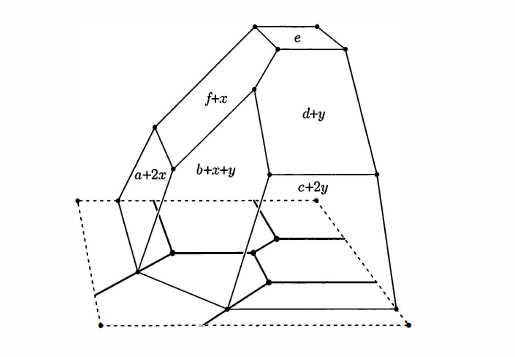
\includegraphics[width=15cm]{./figures/tent-over-R2.png}
    \caption{Tent over $\bR^2$}
    \label{fig:tent-over-R2}
\end{figure}

\begin{prop}\label{prop:finite-embedded-graph}
  The polynomial $V(p) \subseteq \bR^2$ is a finite embedded graph (with bounded and unbounded edges) and all edge slopes are rational. Moreoever, each edge $E$ of $V(p)$ comes with a weight $w(E) \in \bN\setminus \{0\}$ such that at each vertex $v \in V(p)$ we have
  \begin{align*}
    \sum w(E)\cdot u_{V,E} = 0.
  \end{align*}
  This is called the \textbf{balancing condition}. The element $u_{V,E} \in \bZ^n$ is a primitive vector in the direction $E$.
\end{prop}
\begin{example}\label{example:looking-closely-at-conic}
  
\end{example}
\subsection{Relation to subdivisions of the Newton polygon}
Let $p = \bigoplus_{I\subseteq \bZ^2} a_I \odot x^I$.
\begin{align*}
  \Newt(p) = \conv \{I\in I^2 \subseteq \bR^2 ~\mid~ a_I \neq \infty\} \subseteq \bR^2
\end{align*}

\begin{example}\label{example:a-conic}
  Suppose $p(x) = 1\odot x^2 \oplus 0\odot xy\oplus 1\odot y^2 \oplus 0\odot y\oplus 1$. The $a_I$ provide a function 
  \begin{align*}
    a:\Newt(p) \cap \bZ^2 \to \bR \cup \{\infty\}, 
  \end{align*}
  Given by $I\mapsto a_I$. Take the ``overgraph of $a$'' = $\conv\{(I,a_I) \in \bR^3~\mid~ I\in \Newt(p) \cap \bZ^2\} + \bR_{\geq 0}\cdot (0,0,1)$. The lower body is the union of bd. cells of boundary which is equal to the graph of a piecewise affine function $\varphi:\Newt(p) \to \bR$
\end{example}

Domains of affine linearity of $\varphi$ define a polydral decomposition $P$ of $\Newt(p)$ into convex polyhedra with integral vertices. In the previous example, $V(p)$ is dual to $\Newt(p)$. Furthermore, the edges in the interior of $\Newt(p)$ correspond to bounded edges in $V(p)$ and the boundary edges of $\Newt(p)$ correspond to the unbounded edges of $V(p)$.

\begin{prop}\label{prop:newton-to-tropical-hypersurface}
  $V(p)$ is combinatorially the dual complex of the $1$-skeleton of $P$. Edges in $\partial \Newt(p)$ correspond to unbounded edges (tentacles) of $V(p)$. Edge directions $u_{V,E}$ are the interior normal vectors to the $2$-cell dual to $v$ at the edge dual to $E$.
\end{prop}
\begin{example}\label{example:biquadratic-curves}
  Fill in
\end{example}

This proposition connecting Newton polygons to $V(p)$ also explains the balancing condition. Vertices $v \in V(p)$ is dual to a convex polygon $\sigma \in P$ with integral vertices correspond precisely to slopes of the affine functions defining $V(p)$ locally at $p$. The balancing condition holds if and only if the sum of the edge vectors of $\sigma$ are close to a polygon.

Weights = integral lengths of edge $w = \#(w \cap \bZ^2)$.

\textbf{Note:} Subdivision into standard simplicies ($n = 2$: std $\iff $ Area = $\frac{1}{2}$)

\subsection{Intersections of plane tropical curves}

\begin{thm}[Bezout's Theorem]\label{thm:bezout-thm}
  Suppose $f_1,f_2 \in \bC[x,y,z]$ are homogeneous of degree $d_i > 0$. Suppose also that $f_i$ is irreducible and that for $c \in \bC$ $f_i = cf_j \implies i = j$. Then the degree $d$ algebraic curve
  \begin{align*}
    C_i = V(f_i) = \{[x:y:z] \in \bP^2_\bC ~\mid~ f_i(x,y,z) = 0\}
  \end{align*}
  has intersection number $d_id_j$ with $C_j$, i.e. $C_i \# C_j = d_1\cdot d_2$. More precisely, \begin{align*}
    C_i\# C_j = \#(C_i^c \cap C^j)
  \end{align*}
  if $V(f_1^c) = C_i^c$ is a small perurbation of $C_i$.
\end{thm}
\printbibliography
\end{document}
